\section{Evaluation}
Code formatting is inherently a subjective topic.
This introduces a challenge when evaluating a code formatter.
In this chapter, we will present measurements that we believe show the success of scalafmt.
We do not measure how well software developers perceive scalafmt formatted code.
Instead, we will focus on \emph{performance benchmarks} and \emph{user adoption}.

\subsection{Performance benchmarks}
In this chapter, we describe our test methodology, key metrics and the performance results.

\subsubsection{Hardware}
The benchmarks are run on a Macbook Pro (Retina, 15-inch, Mid 2014) laptop with a quad-core 2.5 GHz Intel Core i7 processor, 256 KB L2 cache per core and 6 MB shared L3 cache.
The laptop has 16 GB 1600 MHz DDR3 memory.
The operating system is OS X El Capitan 10.11.5.
We run the benchmarks from the scalafmt commit id \href{https://github.com/olafurpg/scalafmt/tree/aff5e794dae4787b08243f8abb87a3ca4d907e40}{aff5e794} compiled against Scala 2.11.7, running on JVM version 8, update 91.

\subsubsection{Macro benchmark}
The macro benchmarks is designed to get insight on how scalafmt performs in a continuous integration setup.
We format 9.423 source files taken from a subset of seven projects from the property based testing inputs\footnote{
  Download here \url{https://github.com/olafurpg/scalafmt/releases/download/v0.1.4/repos.tar.gz}
}: intellij-scala, akka, spark, scalding, fastparse, scala-js and goose.
The whole sample contains over 1.2 million lines of code --- orders of magnitude larger than what a continuous integration server typically tests for code review.
Table~\ref{tab:macro_sample} shows the distribution of file sizes.
\begin{table}
  \centering
  \begin{tabular}{llllllll}
  25th & Median & Mean & 75th & 90th & 95th & 99th & Max\\
  \hline
  \hline
  16 & 46 & 106 & 113 & 248 & 400 & 945 & 11.723\\
  
\end{tabular}

  \caption{Percentiles of lines of code per file in macro benchmark.}~\label{tab:macro_sample}
\end{table}
For example, 25th percentile of files have 16 lines of code.
Observe that over 90 percent of all files are rather small, or under 300 lines of code.
Less than one percent of all files contain over 1.000 lines of code.
For accurate measurements, we run five iterations of the macro benchmark.
We compare the running time with Scalariform.
The macro benchmark is multi-threaded and takes advantage of all cores on the underlying hardware.

Table~\ref{tab:macro} shows the results from the macro benchmark.
\begin{table}
  \centering
  \begin{tabular}{lllll}
  Benchmark                &  Cores  &   Score  &   Error &  Units\\
  \hline
  \hline
  Parallel.scalafmt        &  4      &  14.616  &   0.632 &   s/op\\
  Parallel.scalariform     &  4      &   2.810  &   0.641 &   s/op\\
\hline
  Ratio &  & 5.20 &  & \\
  \\
  Synchronous.scalafmt     &  1      &  35.654  &   0.459 &   s/op\\
  Synchronous.scalariform  &  1      &   5.951  &   0.135 &   s/op\\
\hline
  Ratio &  & 5.99 &  & 
\end{tabular}

  \caption{Results from macro benchmark.}\label{tab:macro}
\end{table}
Scalafmt is much slower, which may not be surprising considering since scalafmt's primary goal has always been to produce appealing output.
Scalafmt may try thousands of different formatting layouts to produce an optimal formatting output.
Scalariform's formatting algorithm is linear.
Still, we are quite content with the performance of scalafmt.
This benchmark reveals that scalafmt can format 12.000 lines of code per second.


\subsubsection{Micro benchmark}
The micro benchmark is designed to get insight into how scalafmt performs in an interactive software developer workflow.
For example, it is common to configure a text editor to format source code on every save.
We select four files of varying sizes: small ($\sim$ 50 LOC), medium ($\sim$300 LOC), large ($\sim$1.000 LOC) and extra large ($\sim$4.500 LOC).
Recall that over 90\% of all source files in the macro benchmarks were medium sized or smaller, as revealed by table~\ref{tab:macro_sample}.
Because of the fine granularity in this benchmark, we use the OpenJDK Java Microbenchmark Harness (JMH)\autocite{OpenJ38:online}.
JMH accounts for \texttt{nanoTime} overhead and a variety of other parameters that affect performance on the JVM.
To minimize error margins, we run 10 warmup iterations followed by 10 measured iterations.
The sbt-jmh\autocite{ktoso84:online} plugin makes it easy to integrate JMH with a Scala project.
As in the macro benchmark, we compare the running time with Scalariform.
The micro benchmark is single threaded.

Table~\ref{tab:micro} shows the results from the micro benchmark.
\begin{table}
  \centering
  \input{target/micro.tex}
  \caption{Results from micro benchmark.}\label{tab:micro}
\end{table}
No surprise, scalafmt is a slower than Scalariform again.
In fact, scalafmt seems a lot slower in this benchmark compared to the macro benchmark.
Why is that?
Moreover, is this performance gap acceptable for interactive software development.

To answer the first question, we believe scalafmt performs better in the macro benchmark --- relative to Scalariform --- because macro benchmark is multi-threaded while the micro benchmark is single threaded.
As the measurements show, scalafmt operations are slower.
Hence, the scheduler in the macro benchmark is presumably more efficient at allocating CPU wall time to the scalafmt test runs compared to Scalariform.

Secondly, we believe this performance is usable for most use-cases, but needs improvements to be acceptable for settings such as reformat on save/compile.
We currently don't recommend users to configure text editors to run scalafmt no every file save.
Amazon famously showed that sales decreased by 1 percent for every 100ms increase in page load time\autocite{kohavi2007online}.
We believe similar principles apply to scalafmt, every millisecond counts in the user experience.
Still, we believe with the current performance scalafmt delivers enough benefits to be useful.
As we'll discuss in the following section, our users seem to agree.

\subsection{Adoption}\label{sec:adoption}
Scalafmt has received quite some attention since its release in early March, three months ago.
In this section we present the statistics we believe demonstrate that scalafmt is --- despite its young age --- already proving itself useful for the Scala community.

\begin{itemize}
  \item Scalafmt has been installed over 6.500 times.
    Table~\ref{tab:installs} shows the installation numbers for each official distribution channel.
    \begin{table}
      \centering
      \begin{tabular}{lll}
  Channel          & Version  &  Installations\\
  \hline
  \hline
  IntelliJ         & v0.2.5   &  847            \\
                   & All      &  3.273\\
  Maven            & v0.2.5   &  788            \\
                   & All      &  2.657          \\
  Github           & v0.2.5   &  102            \\
                   & All      &  929            \\
\hline
  Sum        & v0.2.5   &  1.737          \\
                   & All      &  6.859          
\end{tabular}

      \caption{Download numbers for scalafmt as of June 9th 2016.}\label{tab:installs}
    \end{table}
    \begin{figure}
      \centering
      \includegraphics[width=0.4\textwidth,angle=-90]{target/month.eps}
      \caption{Download numbers for scalafmt as of June 9th 2016.}\label{tab:installs}
    \end{figure}
    Observe that v0.2.5 was released 22 days ago.
    Also, consider that those
\end{itemize}



